\documentclass[1p]{elsarticle_modified}
%\bibliographystyle{elsarticle-num}

%\usepackage[colorlinks]{hyperref}
%\usepackage{abbrmath_seonhwa} %\Abb, \Ascr, \Acal ,\Abf, \Afrak
\usepackage{amsfonts}
\usepackage{amssymb}
\usepackage{amsmath}
\usepackage{amsthm}
\usepackage{scalefnt}
\usepackage{amsbsy}
\usepackage{kotex}
\usepackage{caption}
\usepackage{subfig}
\usepackage{color}
\usepackage{graphicx}
\usepackage{xcolor} %% white, black, red, green, blue, cyan, magenta, yellow
\usepackage{float}
\usepackage{setspace}
\usepackage{hyperref}

\usepackage{tikz}
\usetikzlibrary{arrows}

\usepackage{multirow}
\usepackage{array} % fixed length table
\usepackage{hhline}

%%%%%%%%%%%%%%%%%%%%%
\makeatletter
\renewcommand*\env@matrix[1][\arraystretch]{%
	\edef\arraystretch{#1}%
	\hskip -\arraycolsep
	\let\@ifnextchar\new@ifnextchar
	\array{*\c@MaxMatrixCols c}}
\makeatother %https://tex.stackexchange.com/questions/14071/how-can-i-increase-the-line-spacing-in-a-matrix
%%%%%%%%%%%%%%%

\usepackage[normalem]{ulem}

\newcommand{\msout}[1]{\ifmmode\text{\sout{\ensuremath{#1}}}\else\sout{#1}\fi}
%SOURCE: \msout is \stkout macro in https://tex.stackexchange.com/questions/20609/strikeout-in-math-mode

\newcommand{\cancel}[1]{
	\ifmmode
	{\color{red}\msout{#1}}
	\else
	{\color{red}\sout{#1}}
	\fi
}

\newcommand{\add}[1]{
	{\color{blue}\uwave{#1}}
}

\newcommand{\replace}[2]{
	\ifmmode
	{\color{red}\msout{#1}}{\color{blue}\uwave{#2}}
	\else
	{\color{red}\sout{#1}}{\color{blue}\uwave{#2}}
	\fi
}

\newcommand{\Sol}{\mathcal{S}} %segment
\newcommand{\D}{D} %diagram
\newcommand{\A}{\mathcal{A}} %arc


%%%%%%%%%%%%%%%%%%%%%%%%%%%%%5 test

\def\sl{\operatorname{\textup{SL}}(2,\Cbb)}
\def\psl{\operatorname{\textup{PSL}}(2,\Cbb)}
\def\quan{\mkern 1mu \triangleright \mkern 1mu}

\theoremstyle{definition}
\newtheorem{thm}{Theorem}[section]
\newtheorem{prop}[thm]{Proposition}
\newtheorem{lem}[thm]{Lemma}
\newtheorem{ques}[thm]{Question}
\newtheorem{cor}[thm]{Corollary}
\newtheorem{defn}[thm]{Definition}
\newtheorem{exam}[thm]{Example}
\newtheorem{rmk}[thm]{Remark}
\newtheorem{alg}[thm]{Algorithm}

\newcommand{\I}{\sqrt{-1}}
\begin{document}

%\begin{frontmatter}
%
%\title{Boundary parabolic representations of knots up to 8 crossings}
%
%%% Group authors per affiliation:
%\author{Yunhi Cho} 
%\address{Department of Mathematics, University of Seoul, Seoul, Korea}
%\ead{yhcho@uos.ac.kr}
%
%
%\author{Seonhwa Kim} %\fnref{s_kim}}
%\address{Center for Geometry and Physics, Institute for Basic Science, Pohang, 37673, Korea}
%\ead{ryeona17@ibs.re.kr}
%
%\author{Hyuk Kim}
%\address{Department of Mathematical Sciences, Seoul National University, Seoul 08826, Korea}
%\ead{hyukkim@snu.ac.kr}
%
%\author{Seokbeom Yoon}
%\address{Department of Mathematical Sciences, Seoul National University, Seoul, 08826,  Korea}
%\ead{sbyoon15@snu.ac.kr}
%
%\begin{abstract}
%We find all boundary parabolic representation of knots up to 8 crossings.
%
%\end{abstract}
%\begin{keyword}
%    \MSC[2010] 57M25 
%\end{keyword}
%
%\end{frontmatter}

%\linenumbers
%\tableofcontents
%
\newcommand\colored[1]{\textcolor{white}{\rule[-0.35ex]{0.8em}{1.4ex}}\kern-0.8em\color{red} #1}%
%\newcommand\colored[1]{\textcolor{white}{ #1}\kern-2.17ex	\textcolor{white}{ #1}\kern-1.81ex	\textcolor{white}{ #1}\kern-2.15ex\color{red}#1	}

{\Large $\underline{12a_{0737}~(K12a_{0737})}$}

\setlength{\tabcolsep}{10pt}
\renewcommand{\arraystretch}{1.6}
\vspace{1cm}\begin{tabular}{m{100pt}>{\centering\arraybackslash}m{274pt}}
\multirow{5}{120pt}{
	\centering
	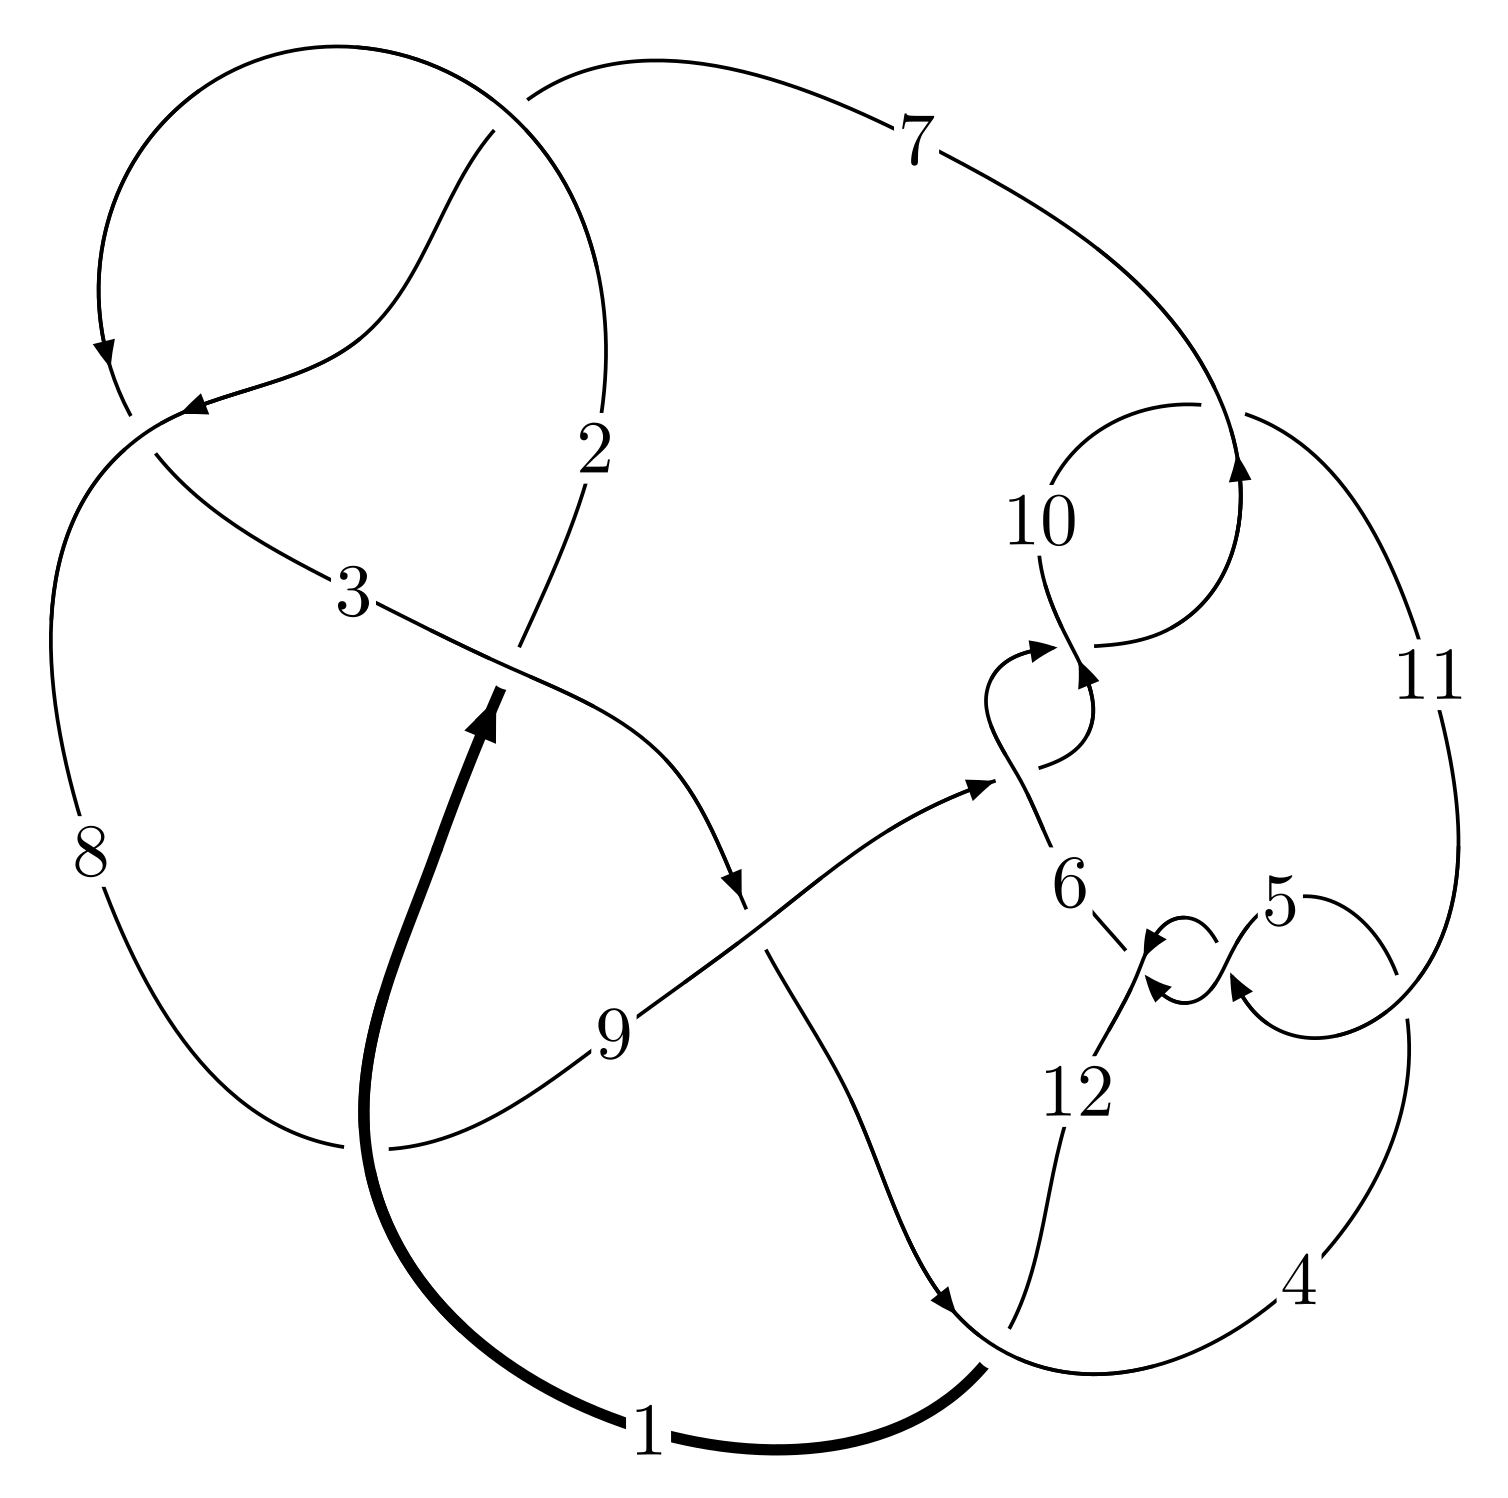
\includegraphics[width=112pt]{../../../GIT/diagram.site/Diagrams/png/1538_12a_0737.png}\\
\ \ \ A knot diagram\footnotemark}&
\allowdisplaybreaks
\textbf{Linearized knot diagam} \\
\cline{2-2}
 &
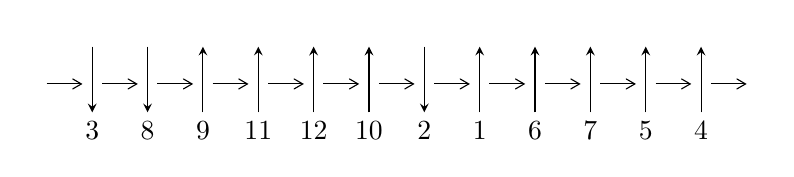
\begin{tikzpicture}[x=20pt, y=17pt]
	% nodes
	\node (C0) at (0, 0) {};
	\node (C1) at (1, 0) {};
	\node (C1U) at (1, +1) {};
	\node (C1D) at (1, -1) {3};

	\node (C2) at (2, 0) {};
	\node (C2U) at (2, +1) {};
	\node (C2D) at (2, -1) {8};

	\node (C3) at (3, 0) {};
	\node (C3U) at (3, +1) {};
	\node (C3D) at (3, -1) {9};

	\node (C4) at (4, 0) {};
	\node (C4U) at (4, +1) {};
	\node (C4D) at (4, -1) {11};

	\node (C5) at (5, 0) {};
	\node (C5U) at (5, +1) {};
	\node (C5D) at (5, -1) {12};

	\node (C6) at (6, 0) {};
	\node (C6U) at (6, +1) {};
	\node (C6D) at (6, -1) {10};

	\node (C7) at (7, 0) {};
	\node (C7U) at (7, +1) {};
	\node (C7D) at (7, -1) {2};

	\node (C8) at (8, 0) {};
	\node (C8U) at (8, +1) {};
	\node (C8D) at (8, -1) {1};

	\node (C9) at (9, 0) {};
	\node (C9U) at (9, +1) {};
	\node (C9D) at (9, -1) {6};

	\node (C10) at (10, 0) {};
	\node (C10U) at (10, +1) {};
	\node (C10D) at (10, -1) {7};

	\node (C11) at (11, 0) {};
	\node (C11U) at (11, +1) {};
	\node (C11D) at (11, -1) {5};

	\node (C12) at (12, 0) {};
	\node (C12U) at (12, +1) {};
	\node (C12D) at (12, -1) {4};
	\node (C13) at (13, 0) {};

	% arrows
	\draw[->,>={angle 60}]
	(C0) edge (C1) (C1) edge (C2) (C2) edge (C3) (C3) edge (C4) (C4) edge (C5) (C5) edge (C6) (C6) edge (C7) (C7) edge (C8) (C8) edge (C9) (C9) edge (C10) (C10) edge (C11) (C11) edge (C12) (C12) edge (C13) ;	\draw[->,>=stealth]
	(C1U) edge (C1D) (C2U) edge (C2D) (C3D) edge (C3U) (C4D) edge (C4U) (C5D) edge (C5U) (C6D) edge (C6U) (C7U) edge (C7D) (C8D) edge (C8U) (C9D) edge (C9U) (C10D) edge (C10U) (C11D) edge (C11U) (C12D) edge (C12U) ;
	\end{tikzpicture} \\
\hhline{~~} \\& 
\textbf{Solving Sequence} \\ \cline{2-2} 
 &
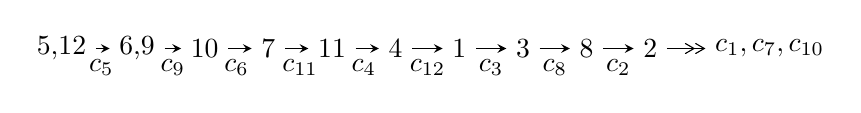
\begin{tikzpicture}[x=23pt, y=7pt]
	% node
	\node (A0) at (-1/8, 0) {5,12};
	\node (A1) at (17/16, 0) {6,9};
	\node (A2) at (17/8, 0) {10};
	\node (A3) at (25/8, 0) {7};
	\node (A4) at (33/8, 0) {11};
	\node (A5) at (41/8, 0) {4};
	\node (A6) at (49/8, 0) {1};
	\node (A7) at (57/8, 0) {3};
	\node (A8) at (65/8, 0) {8};
	\node (A9) at (73/8, 0) {2};
	\node (C1) at (1/2, -1) {$c_{5}$};
	\node (C2) at (13/8, -1) {$c_{9}$};
	\node (C3) at (21/8, -1) {$c_{6}$};
	\node (C4) at (29/8, -1) {$c_{11}$};
	\node (C5) at (37/8, -1) {$c_{4}$};
	\node (C6) at (45/8, -1) {$c_{12}$};
	\node (C7) at (53/8, -1) {$c_{3}$};
	\node (C8) at (61/8, -1) {$c_{8}$};
	\node (C9) at (69/8, -1) {$c_{2}$};
	\node (A10) at (11, 0) {$c_{1},c_{7},c_{10}$};

	% edge
	\draw[->,>=stealth]	
	(A0) edge (A1) (A1) edge (A2) (A2) edge (A3) (A3) edge (A4) (A4) edge (A5) (A5) edge (A6) (A6) edge (A7) (A7) edge (A8) (A8) edge (A9) ;
	\draw[->>,>={angle 60}]	
	(A9) edge (A10);
\end{tikzpicture} \\ 

\end{tabular} \\

\footnotetext{
The image of knot diagram is generated by the software ``\textbf{Draw programme}" developed by Andrew Bartholomew(\url{http://www.layer8.co.uk/maths/draw/index.htm\#Running-draw}), where we modified some parts for our purpose(\url{https://github.com/CATsTAILs/LinksPainter}).
}\phantom \\ \newline 
\centering \textbf{Ideals for irreducible components\footnotemark of $X_{\text{par}}$} 
 
\begin{align*}
I^u_{1}&=\langle 
u^{34}- u^{33}+\cdots+8 b-7 u,\;- u^{34}+u^{33}+\cdots+8 a+23 u,\;u^{35}- u^{34}+\cdots+5 u^2-1\rangle \\
I^u_{2}&=\langle 
3 u^{13}- u^{12}-22 u^{11}+11 u^{10}+49 u^9-17 u^8-35 u^7-15 u^6-4 u^5+45 u^4+8 u^3-16 u^2+11 b-2 u-9,\\
\phantom{I^u_{2}}&\phantom{= \langle  }5 u^{13}+2 u^{12}-22 u^{11}-11 u^{10}+34 u^9+23 u^8-7 u^7-25 u^6-36 u^5+20 u^4+39 u^3- u^2+11 a-7 u-15,\\
\phantom{I^u_{2}}&\phantom{= \langle  }u^{14}-5 u^{12}+9 u^{10}+u^9-5 u^8-4 u^7-3 u^6+6 u^5+4 u^4-2 u^3-2 u-1\rangle \\
I^u_{3}&=\langle 
48312506401 u^{39}-25481530594 u^{38}+\cdots+43198696939 b-277160237401,\\
\phantom{I^u_{3}}&\phantom{= \langle  }-199007192694 u^{39}+322170993904 u^{38}+\cdots+215993484695 a+1742428011421,\\
\phantom{I^u_{3}}&\phantom{= \langle  }u^{40}- u^{39}+\cdots+6 u+5\rangle \\
I^u_{4}&=\langle 
b+a-1,\;a^4+2 a^2+2,\;u+1\rangle \\
I^u_{5}&=\langle 
b+a+1,\;a^3,\;u-1\rangle \\
\\
\end{align*}
\raggedright * 5 irreducible components of $\dim_{\mathbb{C}}=0$, with total 96 representations.\\
\footnotetext{All coefficients of polynomials are rational numbers. But the coefficients are sometimes approximated in decimal forms when there is not enough margin.}
\newpage
\renewcommand{\arraystretch}{1}
\centering \section*{I. $I^u_{1}= \langle u^{34}- u^{33}+\cdots+8 b-7 u,\;- u^{34}+u^{33}+\cdots+8 a+23 u,\;u^{35}- u^{34}+\cdots+5 u^2-1 \rangle$}
\flushleft \textbf{(i) Arc colorings}\\
\begin{tabular}{m{7pt} m{180pt} m{7pt} m{180pt} }
\flushright $a_{5}=$&$\begin{pmatrix}1\\0\end{pmatrix}$ \\
\flushright $a_{12}=$&$\begin{pmatrix}0\\u\end{pmatrix}$ \\
\flushright $a_{6}=$&$\begin{pmatrix}1\\- u^2\end{pmatrix}$ \\
\flushright $a_{9}=$&$\begin{pmatrix}\frac{1}{8} u^{34}-\frac{1}{8} u^{33}+\cdots-\frac{5}{2} u^3-\frac{23}{8} u\\-\frac{1}{8} u^{34}+\frac{1}{8} u^{33}+\cdots+\frac{7}{2} u^3+\frac{7}{8} u\end{pmatrix}$ \\
\flushright $a_{10}=$&$\begin{pmatrix}\frac{1}{8} u^{34}-\frac{1}{8} u^{33}+\cdots-\frac{5}{2} u^3-\frac{15}{8} u\\-\frac{1}{8} u^{34}+\frac{1}{8} u^{33}+\cdots+\frac{5}{2} u^3+\frac{7}{8} u\end{pmatrix}$ \\
\flushright $a_{7}=$&$\begin{pmatrix}-\frac{1}{8} u^{33}+\frac{1}{8} u^{32}+\cdots+\frac{5}{2} u^2+\frac{7}{8}\\\frac{1}{8} u^{33}-\frac{1}{8} u^{32}+\cdots-\frac{5}{2} u^2+\frac{1}{8}\end{pmatrix}$ \\
\flushright $a_{11}=$&$\begin{pmatrix}- u\\u\end{pmatrix}$ \\
\flushright $a_{4}=$&$\begin{pmatrix}- u^2+1\\u^2\end{pmatrix}$ \\
\flushright $a_{1}=$&$\begin{pmatrix}u^5-2 u^3+u\\- u^5+u^3+u\end{pmatrix}$ \\
\flushright $a_{3}=$&$\begin{pmatrix}-\frac{1}{8} u^{34}-\frac{1}{4} u^{33}+\cdots-\frac{1}{8} u+\frac{7}{8}\\\frac{1}{8} u^{34}+\frac{3}{8} u^{33}+\cdots+\frac{1}{8} u+\frac{1}{4}\end{pmatrix}$ \\
\flushright $a_{8}=$&$\begin{pmatrix}\frac{1}{8} u^{34}-\frac{1}{8} u^{33}+\cdots-\frac{13}{2} u^3-\frac{23}{8} u\\u^{13}-5 u^{11}+7 u^9+2 u^7-8 u^5- u^3+u\end{pmatrix}$ \\
\flushright $a_{2}=$&$\begin{pmatrix}\frac{1}{8} u^{34}- u^{33}+\cdots+\frac{13}{8} u-\frac{7}{8}\\\frac{1}{4} u^{34}+\frac{7}{8} u^{33}+\cdots-\frac{13}{4} u^2+\frac{7}{8}\end{pmatrix}$\\&\end{tabular}
\flushleft \textbf{(ii) Obstruction class $= -1$}\\~\\
\flushleft \textbf{(iii) Cusp Shapes $= \frac{3}{4} u^{34}+\frac{1}{4} u^{33}+\cdots+\frac{49}{4} u+\frac{15}{2}$}\\~\\
\newpage\renewcommand{\arraystretch}{1}
\flushleft \textbf{(iv) u-Polynomials at the component}\newline \\
\begin{tabular}{m{50pt}|m{274pt}}
Crossings & \hspace{64pt}u-Polynomials at each crossing \\
\hline $$\begin{aligned}c_{1}\end{aligned}$$&$\begin{aligned}
&u^{35}+17 u^{34}+\cdots+4 u+4
\end{aligned}$\\
\hline $$\begin{aligned}c_{2},c_{7}\end{aligned}$$&$\begin{aligned}
&u^{35}+3 u^{34}+\cdots+6 u+2
\end{aligned}$\\
\hline $$\begin{aligned}c_{3}\end{aligned}$$&$\begin{aligned}
&u^{35}-3 u^{34}+\cdots+72 u+296
\end{aligned}$\\
\hline $$\begin{aligned}c_{4},c_{5},c_{6}\\c_{9},c_{10},c_{11}\end{aligned}$$&$\begin{aligned}
&u^{35}- u^{34}+\cdots+5 u^2-1
\end{aligned}$\\
\hline $$\begin{aligned}c_{8}\end{aligned}$$&$\begin{aligned}
&u^{35}+9 u^{34}+\cdots-70 u-46
\end{aligned}$\\
\hline $$\begin{aligned}c_{12}\end{aligned}$$&$\begin{aligned}
&u^{35}+3 u^{34}+\cdots+256 u+256
\end{aligned}$\\
\hline
\end{tabular}\\~\\
\newpage\renewcommand{\arraystretch}{1}
\flushleft \textbf{(v) Riley Polynomials at the component}\newline \\
\begin{tabular}{m{50pt}|m{274pt}}
Crossings & \hspace{64pt}Riley Polynomials at each crossing \\
\hline $$\begin{aligned}c_{1}\end{aligned}$$&$\begin{aligned}
&y^{35}+3 y^{34}+\cdots-240 y-16
\end{aligned}$\\
\hline $$\begin{aligned}c_{2},c_{7}\end{aligned}$$&$\begin{aligned}
&y^{35}-17 y^{34}+\cdots+4 y-4
\end{aligned}$\\
\hline $$\begin{aligned}c_{3}\end{aligned}$$&$\begin{aligned}
&y^{35}- y^{34}+\cdots+704928 y-87616
\end{aligned}$\\
\hline $$\begin{aligned}c_{4},c_{5},c_{6}\\c_{9},c_{10},c_{11}\end{aligned}$$&$\begin{aligned}
&y^{35}-37 y^{34}+\cdots+10 y-1
\end{aligned}$\\
\hline $$\begin{aligned}c_{8}\end{aligned}$$&$\begin{aligned}
&y^{35}+11 y^{34}+\cdots+28820 y-2116
\end{aligned}$\\
\hline $$\begin{aligned}c_{12}\end{aligned}$$&$\begin{aligned}
&y^{35}+7 y^{34}+\cdots+1441792 y-65536
\end{aligned}$\\
\hline
\end{tabular}\\~\\
\newpage\flushleft \textbf{(vi) Complex Volumes and Cusp Shapes}
$$\begin{array}{c|c|c}  
\text{Solutions to }I^u_{1}& \I (\text{vol} + \sqrt{-1}CS) & \text{Cusp shape}\\
 \hline 
\begin{aligned}
u &= -0.167828 + 0.756763 I \\
a &= \phantom{-}0.22251 - 1.74569 I \\
b &= \phantom{-}0.396759 - 0.137285 I\end{aligned}
 & -4.21898 - 7.81840 I & \phantom{-}0.96471 + 7.49925 I \\ \hline\begin{aligned}
u &= -0.167828 - 0.756763 I \\
a &= \phantom{-}0.22251 + 1.74569 I \\
b &= \phantom{-}0.396759 + 0.137285 I\end{aligned}
 & -4.21898 + 7.81840 I & \phantom{-}0.96471 - 7.49925 I \\ \hline\begin{aligned}
u &= -0.086793 + 0.752466 I \\
a &= \phantom{-}0.11704 - 1.72052 I \\
b &= \phantom{-}0.203323 - 0.193454 I\end{aligned}
 & -5.93777 - 0.09592 I & -2.21151 + 0.44008 I \\ \hline\begin{aligned}
u &= -0.086793 - 0.752466 I \\
a &= \phantom{-}0.11704 + 1.72052 I \\
b &= \phantom{-}0.203323 + 0.193454 I\end{aligned}
 & -5.93777 + 0.09592 I & -2.21151 - 0.44008 I \\ \hline\begin{aligned}
u &= \phantom{-}0.152216 + 0.717373 I \\
a &= -0.21415 - 1.68842 I \\
b &= -0.321763 - 0.065640 I\end{aligned}
 & -1.80618 + 3.02164 I & \phantom{-}3.90973 - 3.95401 I \\ \hline\begin{aligned}
u &= \phantom{-}0.152216 - 0.717373 I \\
a &= -0.21415 + 1.68842 I \\
b &= -0.321763 + 0.065640 I\end{aligned}
 & -1.80618 - 3.02164 I & \phantom{-}3.90973 + 3.95401 I \\ \hline\begin{aligned}
u &= -1.300490 + 0.187880 I \\
a &= -1.52389 - 1.71909 I \\
b &= \phantom{-}2.06311 + 2.28997 I\end{aligned}
 & \phantom{-}2.41004 + 1.41249 I & \phantom{-}9.47570 + 0. I\phantom{ +0.000000I} \\ \hline\begin{aligned}
u &= -1.300490 - 0.187880 I \\
a &= -1.52389 + 1.71909 I \\
b &= \phantom{-}2.06311 - 2.28997 I\end{aligned}
 & \phantom{-}2.41004 - 1.41249 I & \phantom{-}9.47570 + 0. I\phantom{ +0.000000I} \\ \hline\begin{aligned}
u &= -1.311970 + 0.248425 I \\
a &= -1.07722 - 1.85643 I \\
b &= \phantom{-}1.68583 + 2.62705 I\end{aligned}
 & \phantom{-}1.60231 - 6.99533 I & \phantom{-}7.54634 + 6.51965 I \\ \hline\begin{aligned}
u &= -1.311970 - 0.248425 I \\
a &= -1.07722 + 1.85643 I \\
b &= \phantom{-}1.68583 - 2.62705 I\end{aligned}
 & \phantom{-}1.60231 + 6.99533 I & \phantom{-}7.54634 - 6.51965 I\\
 \hline 
 \end{array}$$\newpage$$\begin{array}{c|c|c}  
\text{Solutions to }I^u_{1}& \I (\text{vol} + \sqrt{-1}CS) & \text{Cusp shape}\\
 \hline 
\begin{aligned}
u &= \phantom{-}1.331990 + 0.208218 I \\
a &= \phantom{-}1.25521 - 1.60201 I \\
b &= -1.72921 + 2.28481 I\end{aligned}
 & \phantom{-}5.46888 + 3.18024 I & \phantom{-}12.51891 - 3.03421 I \\ \hline\begin{aligned}
u &= \phantom{-}1.331990 - 0.208218 I \\
a &= \phantom{-}1.25521 + 1.60201 I \\
b &= -1.72921 - 2.28481 I\end{aligned}
 & \phantom{-}5.46888 - 3.18024 I & \phantom{-}12.51891 + 3.03421 I \\ \hline\begin{aligned}
u &= \phantom{-}0.161198 + 0.551221 I \\
a &= -0.29100 - 1.43200 I \\
b &= -0.174142 + 0.205041 I\end{aligned}
 & -0.34475 + 1.77362 I & \phantom{-}4.56578 - 5.89788 I \\ \hline\begin{aligned}
u &= \phantom{-}0.161198 - 0.551221 I \\
a &= -0.29100 + 1.43200 I \\
b &= -0.174142 - 0.205041 I\end{aligned}
 & -0.34475 - 1.77362 I & \phantom{-}4.56578 + 5.89788 I \\ \hline\begin{aligned}
u &= \phantom{-}1.38810 + 0.33957 I \\
a &= \phantom{-}0.48176 - 1.67486 I \\
b &= -1.06352 + 2.91942 I\end{aligned}
 & \phantom{-}3.48171 + 8.10374 I & \phantom{-}6.00000 - 4.49399 I \\ \hline\begin{aligned}
u &= \phantom{-}1.38810 - 0.33957 I \\
a &= \phantom{-}0.48176 + 1.67486 I \\
b &= -1.06352 - 2.91942 I\end{aligned}
 & \phantom{-}3.48171 - 8.10374 I & \phantom{-}6.00000 + 4.49399 I \\ \hline\begin{aligned}
u &= \phantom{-}1.43331\phantom{ +0.000000I} \\
a &= \phantom{-}1.28549\phantom{ +0.000000I} \\
b &= -1.20757\phantom{ +0.000000I}\end{aligned}
 & \phantom{-}8.30021\phantom{ +0.000000I} & \phantom{-}10.1560\phantom{ +0.000000I} \\ \hline\begin{aligned}
u &= \phantom{-}1.43493 + 0.26536 I \\
a &= \phantom{-}0.64645 - 1.33183 I \\
b &= -0.86486 + 2.42158 I\end{aligned}
 & \phantom{-}9.31625 + 3.51006 I & \phantom{-}13.29415 + 0. I\phantom{ +0.000000I} \\ \hline\begin{aligned}
u &= \phantom{-}1.43493 - 0.26536 I \\
a &= \phantom{-}0.64645 + 1.33183 I \\
b &= -0.86486 - 2.42158 I\end{aligned}
 & \phantom{-}9.31625 - 3.51006 I & \phantom{-}13.29415 + 0. I\phantom{ +0.000000I} \\ \hline\begin{aligned}
u &= -1.41859 + 0.34725 I \\
a &= -0.40165 - 1.57935 I \\
b &= \phantom{-}0.89723 + 2.93938 I\end{aligned}
 & \phantom{-}8.28583 - 11.00080 I & \phantom{-}12.8696 + 5.9885 I\\
 \hline 
 \end{array}$$\newpage$$\begin{array}{c|c|c}  
\text{Solutions to }I^u_{1}& \I (\text{vol} + \sqrt{-1}CS) & \text{Cusp shape}\\
 \hline 
\begin{aligned}
u &= -1.41859 - 0.34725 I \\
a &= -0.40165 + 1.57935 I \\
b &= \phantom{-}0.89723 - 2.93938 I\end{aligned}
 & \phantom{-}8.28583 + 11.00080 I & \phantom{-}12.8696 - 5.9885 I \\ \hline\begin{aligned}
u &= \phantom{-}1.41768 + 0.36311 I \\
a &= \phantom{-}0.35041 - 1.60931 I \\
b &= -0.89725 + 3.02458 I\end{aligned}
 & \phantom{-}5.9000 + 16.1532 I & \phantom{-}9.74356 - 9.72712 I \\ \hline\begin{aligned}
u &= \phantom{-}1.41768 - 0.36311 I \\
a &= \phantom{-}0.35041 + 1.60931 I \\
b &= -0.89725 - 3.02458 I\end{aligned}
 & \phantom{-}5.9000 - 16.1532 I & \phantom{-}9.74356 + 9.72712 I \\ \hline\begin{aligned}
u &= -1.43323 + 0.29831 I \\
a &= -0.53750 - 1.42612 I \\
b &= \phantom{-}0.84249 + 2.64127 I\end{aligned}
 & \phantom{-}10.04470 - 8.52981 I & \phantom{-}14.2743 + 6.4652 I \\ \hline\begin{aligned}
u &= -1.43323 - 0.29831 I \\
a &= -0.53750 + 1.42612 I \\
b &= \phantom{-}0.84249 - 2.64127 I\end{aligned}
 & \phantom{-}10.04470 + 8.52981 I & \phantom{-}14.2743 - 6.4652 I \\ \hline\begin{aligned}
u &= -0.314010 + 0.390794 I \\
a &= \phantom{-}0.71540 - 1.22571 I \\
b &= \phantom{-}0.025527 + 0.500038 I\end{aligned}
 & -1.48480 + 2.02330 I & \phantom{-}2.63866 + 1.25082 I \\ \hline\begin{aligned}
u &= -0.314010 - 0.390794 I \\
a &= \phantom{-}0.71540 + 1.22571 I \\
b &= \phantom{-}0.025527 - 0.500038 I\end{aligned}
 & -1.48480 - 2.02330 I & \phantom{-}2.63866 - 1.25082 I \\ \hline\begin{aligned}
u &= -1.50324 + 0.03422 I \\
a &= -0.874162 - 0.174169 I \\
b &= \phantom{-}0.489019 + 0.337659 I\end{aligned}
 & \phantom{-}13.70520 - 1.40021 I & \phantom{-}16.4192 + 0. I\phantom{ +0.000000I} \\ \hline\begin{aligned}
u &= -1.50324 - 0.03422 I \\
a &= -0.874162 + 0.174169 I \\
b &= \phantom{-}0.489019 - 0.337659 I\end{aligned}
 & \phantom{-}13.70520 + 1.40021 I & \phantom{-}16.4192 + 0. I\phantom{ +0.000000I} \\ \hline\begin{aligned}
u &= -0.450369 + 0.202730 I \\
a &= \phantom{-}1.37562 - 0.88797 I \\
b &= -0.510703 + 0.597542 I\end{aligned}
 & -1.04042 - 4.50619 I & \phantom{-}4.53729 + 8.22316 I\\
 \hline 
 \end{array}$$\newpage$$\begin{array}{c|c|c}  
\text{Solutions to }I^u_{1}& \I (\text{vol} + \sqrt{-1}CS) & \text{Cusp shape}\\
 \hline 
\begin{aligned}
u &= -0.450369 - 0.202730 I \\
a &= \phantom{-}1.37562 + 0.88797 I \\
b &= -0.510703 - 0.597542 I\end{aligned}
 & -1.04042 + 4.50619 I & \phantom{-}4.53729 - 8.22316 I \\ \hline\begin{aligned}
u &= \phantom{-}1.50640 + 0.06553 I \\
a &= \phantom{-}0.834503 - 0.327285 I \\
b &= -0.448322 + 0.642057 I\end{aligned}
 & \phantom{-}12.03530 + 6.55130 I & \phantom{-}13.7606 - 5.2864 I \\ \hline\begin{aligned}
u &= \phantom{-}1.50640 - 0.06553 I \\
a &= \phantom{-}0.834503 + 0.327285 I \\
b &= -0.448322 - 0.642057 I\end{aligned}
 & \phantom{-}12.03530 - 6.55130 I & \phantom{-}13.7606 + 5.2864 I \\ \hline\begin{aligned}
u &= \phantom{-}0.377334 + 0.098062 I \\
a &= -1.222090 - 0.396295 I \\
b &= \phantom{-}0.510257 + 0.241115 I\end{aligned}
 & \phantom{-}0.940032 + 0.385042 I & \phantom{-}10.54272 - 2.65749 I \\ \hline\begin{aligned}
u &= \phantom{-}0.377334 - 0.098062 I \\
a &= -1.222090 + 0.396295 I \\
b &= \phantom{-}0.510257 - 0.241115 I\end{aligned}
 & \phantom{-}0.940032 - 0.385042 I & \phantom{-}10.54272 + 2.65749 I\\
 \hline 
 \end{array}$$\newpage\newpage\renewcommand{\arraystretch}{1}
\centering \section*{II. $I^u_{2}= \langle 3 u^{13}- u^{12}+\cdots+11 b-9,\;5 u^{13}+2 u^{12}+\cdots+11 a-15,\;u^{14}-5 u^{12}+\cdots-2 u-1 \rangle$}
\flushleft \textbf{(i) Arc colorings}\\
\begin{tabular}{m{7pt} m{180pt} m{7pt} m{180pt} }
\flushright $a_{5}=$&$\begin{pmatrix}1\\0\end{pmatrix}$ \\
\flushright $a_{12}=$&$\begin{pmatrix}0\\u\end{pmatrix}$ \\
\flushright $a_{6}=$&$\begin{pmatrix}1\\- u^2\end{pmatrix}$ \\
\flushright $a_{9}=$&$\begin{pmatrix}-0.454545 u^{13}-0.181818 u^{12}+\cdots+0.636364 u+1.36364\\-0.272727 u^{13}+0.0909091 u^{12}+\cdots+0.181818 u+0.818182\end{pmatrix}$ \\
\flushright $a_{10}=$&$\begin{pmatrix}- u^{13}+5 u^{11}-9 u^9- u^8+5 u^7+4 u^6+3 u^5-6 u^4-4 u^3+2 u^2+2\\-0.545455 u^{13}+0.181818 u^{12}+\cdots+0.363636 u+0.636364\end{pmatrix}$ \\
\flushright $a_{7}=$&$\begin{pmatrix}0.636364 u^{13}-0.545455 u^{12}+\cdots+1.90909 u-0.909091\\-1\end{pmatrix}$ \\
\flushright $a_{11}=$&$\begin{pmatrix}- u\\u\end{pmatrix}$ \\
\flushright $a_{4}=$&$\begin{pmatrix}- u^2+1\\u^2\end{pmatrix}$ \\
\flushright $a_{1}=$&$\begin{pmatrix}u^5-2 u^3+u\\- u^5+u^3+u\end{pmatrix}$ \\
\flushright $a_{3}=$&$\begin{pmatrix}-0.818182 u^{13}+0.272727 u^{12}+\cdots+0.545455 u+1.45455\\u^8-2 u^6+u^3+2 u^2- u\end{pmatrix}$ \\
\flushright $a_{8}=$&$\begin{pmatrix}-0.454545 u^{13}-0.181818 u^{12}+\cdots+0.636364 u+1.36364\\-0.272727 u^{13}+0.0909091 u^{12}+\cdots+0.181818 u+0.818182\end{pmatrix}$ \\
\flushright $a_{2}=$&$\begin{pmatrix}-0.727273 u^{13}-0.0909091 u^{12}+\cdots+2.81818 u+1.18182\\0.0909091 u^{13}-0.363636 u^{12}+\cdots+0.272727 u-0.272727\end{pmatrix}$\\&\end{tabular}
\flushleft \textbf{(ii) Obstruction class $= -1$}\\~\\
\flushleft \textbf{(iii) Cusp Shapes $= \frac{16}{11} u^{13}-\frac{20}{11} u^{12}-4 u^{11}+4 u^{10}+\frac{12}{11} u^9+\frac{56}{11} u^8+\frac{48}{11} u^7-\frac{212}{11} u^6-\frac{36}{11} u^5+\frac{108}{11} u^4+\frac{28}{11} u^3+\frac{76}{11} u^2-\frac{40}{11} u+\frac{18}{11}$}\\~\\
\newpage\renewcommand{\arraystretch}{1}
\flushleft \textbf{(iv) u-Polynomials at the component}\newline \\
\begin{tabular}{m{50pt}|m{274pt}}
Crossings & \hspace{64pt}u-Polynomials at each crossing \\
\hline $$\begin{aligned}c_{1}\end{aligned}$$&$\begin{aligned}
&(u^7+4 u^6+8 u^5+8 u^4+4 u^3+u^2+2 u+1)^2
\end{aligned}$\\
\hline $$\begin{aligned}c_{2},c_{7}\end{aligned}$$&$\begin{aligned}
&(u^7-2 u^5+2 u^3+u^2-1)^2
\end{aligned}$\\
\hline $$\begin{aligned}c_{3}\end{aligned}$$&$\begin{aligned}
&(u^7+5 u^6+12 u^5+17 u^4+15 u^3+5 u^2-4 u-4)^2
\end{aligned}$\\
\hline $$\begin{aligned}c_{4},c_{5},c_{6}\\c_{9},c_{10},c_{11}\end{aligned}$$&$\begin{aligned}
&u^{14}-5 u^{12}+9 u^{10}+u^9-5 u^8-4 u^7-3 u^6+6 u^5+4 u^4-2 u^3-2 u-1
\end{aligned}$\\
\hline $$\begin{aligned}c_{8}\end{aligned}$$&$\begin{aligned}
&(u^7+2 u^5+2 u^4+4 u^3+u^2+2 u-1)^2
\end{aligned}$\\
\hline $$\begin{aligned}c_{12}\end{aligned}$$&$\begin{aligned}
&(u^7+2 u^5-2 u^4+4 u^3- u^2+2 u+1)^2
\end{aligned}$\\
\hline
\end{tabular}\\~\\
\newpage\renewcommand{\arraystretch}{1}
\flushleft \textbf{(v) Riley Polynomials at the component}\newline \\
\begin{tabular}{m{50pt}|m{274pt}}
Crossings & \hspace{64pt}Riley Polynomials at each crossing \\
\hline $$\begin{aligned}c_{1}\end{aligned}$$&$\begin{aligned}
&(y^7+8 y^5-4 y^4+24 y^3- y^2+2 y-1)^2
\end{aligned}$\\
\hline $$\begin{aligned}c_{2},c_{7}\end{aligned}$$&$\begin{aligned}
&(y^7-4 y^6+8 y^5-8 y^4+4 y^3- y^2+2 y-1)^2
\end{aligned}$\\
\hline $$\begin{aligned}c_{3}\end{aligned}$$&$\begin{aligned}
&(y^7- y^6+4 y^5+13 y^4- y^3-9 y^2+56 y-16)^2
\end{aligned}$\\
\hline $$\begin{aligned}c_{4},c_{5},c_{6}\\c_{9},c_{10},c_{11}\end{aligned}$$&$\begin{aligned}
&y^{14}-10 y^{13}+\cdots-4 y+1
\end{aligned}$\\
\hline $$\begin{aligned}c_{8},c_{12}\end{aligned}$$&$\begin{aligned}
&(y^7+4 y^6+12 y^5+16 y^4+20 y^3+19 y^2+6 y-1)^2
\end{aligned}$\\
\hline
\end{tabular}\\~\\
\newpage\flushleft \textbf{(vi) Complex Volumes and Cusp Shapes}
$$\begin{array}{c|c|c}  
\text{Solutions to }I^u_{2}& \I (\text{vol} + \sqrt{-1}CS) & \text{Cusp shape}\\
 \hline 
\begin{aligned}
u &= \phantom{-}0.957061 + 0.519308 I \\
a &= \phantom{-}0.514399 + 0.255510 I \\
b &= -1.40007 - 0.49397 I\end{aligned}
 & \phantom{-}5.11553 - 1.84683 I & \phantom{-}13.12815 + 1.09324 I \\ \hline\begin{aligned}
u &= \phantom{-}0.957061 - 0.519308 I \\
a &= \phantom{-}0.514399 - 0.255510 I \\
b &= -1.40007 + 0.49397 I\end{aligned}
 & \phantom{-}5.11553 + 1.84683 I & \phantom{-}13.12815 - 1.09324 I \\ \hline\begin{aligned}
u &= -0.239949 + 0.878713 I \\
a &= -1.07659 + 1.37148 I \\
b &= \phantom{-}0.018151 + 0.213597 I\end{aligned}
 & \phantom{-}0.63279 - 11.68630 I & \phantom{-}6.29693 + 8.84509 I \\ \hline\begin{aligned}
u &= -0.239949 - 0.878713 I \\
a &= -1.07659 - 1.37148 I \\
b &= \phantom{-}0.018151 - 0.213597 I\end{aligned}
 & \phantom{-}0.63279 + 11.68630 I & \phantom{-}6.29693 - 8.84509 I \\ \hline\begin{aligned}
u &= \phantom{-}1.14029\phantom{ +0.000000I} \\
a &= -0.464314\phantom{ +0.000000I} \\
b &= \phantom{-}0.191074\phantom{ +0.000000I}\end{aligned}
 & \phantom{-}2.04041\phantom{ +0.000000I} & \phantom{-}4.35900\phantom{ +0.000000I} \\ \hline\begin{aligned}
u &= -1.168590 + 0.306255 I \\
a &= \phantom{-}0.757257 + 0.859295 I \\
b &= -1.53466 - 1.20028 I\end{aligned}
 & -2.65620 - 3.76357 I & \phantom{-}1.39540 + 4.24459 I \\ \hline\begin{aligned}
u &= -1.168590 - 0.306255 I \\
a &= \phantom{-}0.757257 - 0.859295 I \\
b &= -1.53466 + 1.20028 I\end{aligned}
 & -2.65620 + 3.76357 I & \phantom{-}1.39540 - 4.24459 I \\ \hline\begin{aligned}
u &= -1.321610 + 0.182486 I \\
a &= -0.214561 - 0.416784 I \\
b &= \phantom{-}1.52571 + 1.12991 I\end{aligned}
 & \phantom{-}5.11553 - 1.84683 I & \phantom{-}13.12815 + 1.09324 I \\ \hline\begin{aligned}
u &= -1.321610 - 0.182486 I \\
a &= -0.214561 + 0.416784 I \\
b &= \phantom{-}1.52571 - 1.12991 I\end{aligned}
 & \phantom{-}5.11553 + 1.84683 I & \phantom{-}13.12815 - 1.09324 I \\ \hline\begin{aligned}
u &= \phantom{-}0.043481 + 0.649444 I \\
a &= \phantom{-}1.06596 + 1.83916 I \\
b &= -0.617135 + 0.405783 I\end{aligned}
 & -2.65620 + 3.76357 I & \phantom{-}1.39540 - 4.24459 I\\
 \hline 
 \end{array}$$\newpage$$\begin{array}{c|c|c}  
\text{Solutions to }I^u_{2}& \I (\text{vol} + \sqrt{-1}CS) & \text{Cusp shape}\\
 \hline 
\begin{aligned}
u &= \phantom{-}0.043481 - 0.649444 I \\
a &= \phantom{-}1.06596 - 1.83916 I \\
b &= -0.617135 - 0.405783 I\end{aligned}
 & -2.65620 - 3.76357 I & \phantom{-}1.39540 + 4.24459 I \\ \hline\begin{aligned}
u &= \phantom{-}1.365780 + 0.312423 I \\
a &= -0.455826 + 1.037870 I \\
b &= \phantom{-}1.45156 - 2.32441 I\end{aligned}
 & \phantom{-}0.63279 + 11.68630 I & \phantom{-}6.29693 - 8.84509 I \\ \hline\begin{aligned}
u &= \phantom{-}1.365780 - 0.312423 I \\
a &= -0.455826 - 1.037870 I \\
b &= \phantom{-}1.45156 + 2.32441 I\end{aligned}
 & \phantom{-}0.63279 - 11.68630 I & \phantom{-}6.29693 + 8.84509 I \\ \hline\begin{aligned}
u &= -0.412656\phantom{ +0.000000I} \\
a &= \phantom{-}1.28304\phantom{ +0.000000I} \\
b &= \phantom{-}0.921809\phantom{ +0.000000I}\end{aligned}
 & \phantom{-}2.04041\phantom{ +0.000000I} & \phantom{-}4.35900\phantom{ +0.000000I}\\
 \hline 
 \end{array}$$\newpage\newpage\renewcommand{\arraystretch}{1}
\centering \section*{III. $I^u_{3}= \langle 4.83\times10^{10} u^{39}-2.55\times10^{10} u^{38}+\cdots+4.32\times10^{10} b-2.77\times10^{11},\;-1.99\times10^{11} u^{39}+3.22\times10^{11} u^{38}+\cdots+2.16\times10^{11} a+1.74\times10^{12},\;u^{40}- u^{39}+\cdots+6 u+5 \rangle$}
\flushleft \textbf{(i) Arc colorings}\\
\begin{tabular}{m{7pt} m{180pt} m{7pt} m{180pt} }
\flushright $a_{5}=$&$\begin{pmatrix}1\\0\end{pmatrix}$ \\
\flushright $a_{12}=$&$\begin{pmatrix}0\\u\end{pmatrix}$ \\
\flushright $a_{6}=$&$\begin{pmatrix}1\\- u^2\end{pmatrix}$ \\
\flushright $a_{9}=$&$\begin{pmatrix}0.921357 u^{39}-1.49158 u^{38}+\cdots+14.4435 u-8.06704\\-1.11838 u^{39}+0.589868 u^{38}+\cdots-8.45803 u+6.41594\end{pmatrix}$ \\
\flushright $a_{10}=$&$\begin{pmatrix}\frac{1}{5} u^{39}-\frac{1}{5} u^{38}+\cdots+\frac{24}{5} u+\frac{6}{5}\\-0.721357 u^{39}+1.29158 u^{38}+\cdots-8.64350 u+9.26704\end{pmatrix}$ \\
\flushright $a_{7}=$&$\begin{pmatrix}-1.85341 u^{39}+1.13205 u^{38}+\cdots-56.5699 u-19.7639\\-1\end{pmatrix}$ \\
\flushright $a_{11}=$&$\begin{pmatrix}- u\\u\end{pmatrix}$ \\
\flushright $a_{4}=$&$\begin{pmatrix}- u^2+1\\u^2\end{pmatrix}$ \\
\flushright $a_{1}=$&$\begin{pmatrix}u^5-2 u^3+u\\- u^5+u^3+u\end{pmatrix}$ \\
\flushright $a_{3}=$&$\begin{pmatrix}-0.141219 u^{39}+0.286734 u^{38}+\cdots+12.4150 u+9.11906\\0.874874 u^{39}-1.11047 u^{38}+\cdots+30.2577 u+9.75078\end{pmatrix}$ \\
\flushright $a_{8}=$&$\begin{pmatrix}0.125054 u^{39}-0.909866 u^{38}+\cdots+16.1112 u+2.54657\\-0.585648 u^{39}+1.51958 u^{38}+\cdots-12.9285 u+8.73631\end{pmatrix}$ \\
\flushright $a_{2}=$&$\begin{pmatrix}-1.29679 u^{39}-0.118839 u^{38}+\cdots+35.8131 u+24.9355\\4.70549 u^{39}-0.173819 u^{38}+\cdots-4.96586 u-15.7106\end{pmatrix}$\\&\end{tabular}
\flushleft \textbf{(ii) Obstruction class $= -1$}\\~\\
\flushleft \textbf{(iii) Cusp Shapes $= -\frac{241664643308}{43198696939} u^{39}+\frac{123235657656}{43198696939} u^{38}+\cdots-\frac{438305923412}{43198696939} u+\frac{1059211366526}{43198696939}$}\\~\\
\newpage\renewcommand{\arraystretch}{1}
\flushleft \textbf{(iv) u-Polynomials at the component}\newline \\
\begin{tabular}{m{50pt}|m{274pt}}
Crossings & \hspace{64pt}u-Polynomials at each crossing \\
\hline $$\begin{aligned}c_{1}\end{aligned}$$&$\begin{aligned}
&(u^{20}+9 u^{19}+\cdots+2 u^2+1)^{2}
\end{aligned}$\\
\hline $$\begin{aligned}c_{2},c_{7}\end{aligned}$$&$\begin{aligned}
&(u^{20}- u^{19}+\cdots-2 u+1)^{2}
\end{aligned}$\\
\hline $$\begin{aligned}c_{3}\end{aligned}$$&$\begin{aligned}
&(u^{10}-2 u^9+u^8+4 u^6-6 u^5+u^4+6 u^3-5 u^2+1)^4
\end{aligned}$\\
\hline $$\begin{aligned}c_{4},c_{5},c_{6}\\c_{9},c_{10},c_{11}\end{aligned}$$&$\begin{aligned}
&u^{40}- u^{39}+\cdots+6 u+5
\end{aligned}$\\
\hline $$\begin{aligned}c_{8}\end{aligned}$$&$\begin{aligned}
&(u^{20}-3 u^{19}+\cdots-16 u+5)^{2}
\end{aligned}$\\
\hline $$\begin{aligned}c_{12}\end{aligned}$$&$\begin{aligned}
&(u^{20}+3 u^{19}+\cdots+16 u+5)^{2}
\end{aligned}$\\
\hline
\end{tabular}\\~\\
\newpage\renewcommand{\arraystretch}{1}
\flushleft \textbf{(v) Riley Polynomials at the component}\newline \\
\begin{tabular}{m{50pt}|m{274pt}}
Crossings & \hspace{64pt}Riley Polynomials at each crossing \\
\hline $$\begin{aligned}c_{1}\end{aligned}$$&$\begin{aligned}
&(y^{20}+3 y^{19}+\cdots+4 y+1)^{2}
\end{aligned}$\\
\hline $$\begin{aligned}c_{2},c_{7}\end{aligned}$$&$\begin{aligned}
&(y^{20}-9 y^{19}+\cdots+2 y^2+1)^{2}
\end{aligned}$\\
\hline $$\begin{aligned}c_{3}\end{aligned}$$&$\begin{aligned}
&(y^{10}-2 y^9+\cdots-10 y+1)^{4}
\end{aligned}$\\
\hline $$\begin{aligned}c_{4},c_{5},c_{6}\\c_{9},c_{10},c_{11}\end{aligned}$$&$\begin{aligned}
&y^{40}-31 y^{39}+\cdots+204 y+25
\end{aligned}$\\
\hline $$\begin{aligned}c_{8},c_{12}\end{aligned}$$&$\begin{aligned}
&(y^{20}+3 y^{19}+\cdots+204 y+25)^{2}
\end{aligned}$\\
\hline
\end{tabular}\\~\\
\newpage\flushleft \textbf{(vi) Complex Volumes and Cusp Shapes}
$$\begin{array}{c|c|c}  
\text{Solutions to }I^u_{3}& \I (\text{vol} + \sqrt{-1}CS) & \text{Cusp shape}\\
 \hline 
\begin{aligned}
u &= \phantom{-}0.805245 + 0.548498 I \\
a &= \phantom{-}0.484950 + 0.496101 I \\
b &= -1.063550 - 0.519102 I\end{aligned}
 & \phantom{-}5.84675\phantom{ +0.000000I} & \phantom{-}14.3672 + 0. I\phantom{ +0.000000I} \\ \hline\begin{aligned}
u &= \phantom{-}0.805245 - 0.548498 I \\
a &= \phantom{-}0.484950 - 0.496101 I \\
b &= -1.063550 + 0.519102 I\end{aligned}
 & \phantom{-}5.84675\phantom{ +0.000000I} & \phantom{-}14.3672 + 0. I\phantom{ +0.000000I} \\ \hline\begin{aligned}
u &= -0.729774 + 0.602283 I \\
a &= -0.541328 + 0.641388 I \\
b &= \phantom{-}0.884543 - 0.553467 I\end{aligned}
 & \phantom{-}4.40946 - 4.65452 I & \phantom{-}11.20346 + 6.04247 I \\ \hline\begin{aligned}
u &= -0.729774 - 0.602283 I \\
a &= -0.541328 - 0.641388 I \\
b &= \phantom{-}0.884543 + 0.553467 I\end{aligned}
 & \phantom{-}4.40946 + 4.65452 I & \phantom{-}11.20346 - 6.04247 I \\ \hline\begin{aligned}
u &= -1.066160 + 0.285066 I \\
a &= \phantom{-}0.937984 + 0.759238 I \\
b &= -1.51409 - 0.75635 I\end{aligned}
 & -1.54326 + 3.92983 I & \phantom{-}2.95600 - 3.21471 I \\ \hline\begin{aligned}
u &= -1.066160 - 0.285066 I \\
a &= \phantom{-}0.937984 - 0.759238 I \\
b &= -1.51409 + 0.75635 I\end{aligned}
 & -1.54326 - 3.92983 I & \phantom{-}2.95600 + 3.21471 I \\ \hline\begin{aligned}
u &= \phantom{-}0.254311 + 0.850232 I \\
a &= \phantom{-}1.03350 + 1.37276 I \\
b &= -0.082493 + 0.163450 I\end{aligned}
 & \phantom{-}2.96491 + 6.68616 I & \phantom{-}9.50669 - 5.21994 I \\ \hline\begin{aligned}
u &= \phantom{-}0.254311 - 0.850232 I \\
a &= \phantom{-}1.03350 - 1.37276 I \\
b &= -0.082493 - 0.163450 I\end{aligned}
 & \phantom{-}2.96491 - 6.68616 I & \phantom{-}9.50669 + 5.21994 I \\ \hline\begin{aligned}
u &= -1.041820 + 0.410831 I \\
a &= -0.406675 + 0.084930 I \\
b &= \phantom{-}1.53742 - 0.18333 I\end{aligned}
 & \phantom{-}1.016470 - 0.519983 I & \phantom{-}6.28339 + 0.77505 I \\ \hline\begin{aligned}
u &= -1.041820 - 0.410831 I \\
a &= -0.406675 - 0.084930 I \\
b &= \phantom{-}1.53742 + 0.18333 I\end{aligned}
 & \phantom{-}1.016470 + 0.519983 I & \phantom{-}6.28339 - 0.77505 I\\
 \hline 
 \end{array}$$\newpage$$\begin{array}{c|c|c}  
\text{Solutions to }I^u_{3}& \I (\text{vol} + \sqrt{-1}CS) & \text{Cusp shape}\\
 \hline 
\begin{aligned}
u &= -1.006990 + 0.539596 I \\
a &= -0.566442 + 0.194865 I \\
b &= \phantom{-}1.53566 - 0.53787 I\end{aligned}
 & \phantom{-}2.96491 + 6.68616 I & \phantom{-}9.50669 - 5.21994 I \\ \hline\begin{aligned}
u &= -1.006990 - 0.539596 I \\
a &= -0.566442 - 0.194865 I \\
b &= \phantom{-}1.53566 + 0.53787 I\end{aligned}
 & \phantom{-}2.96491 - 6.68616 I & \phantom{-}9.50669 + 5.21994 I \\ \hline\begin{aligned}
u &= \phantom{-}1.120430 + 0.232272 I \\
a &= -0.796352 + 0.683257 I \\
b &= \phantom{-}1.25298 - 0.91224 I\end{aligned}
 & \phantom{-}1.016470 + 0.519983 I & \phantom{-}6.28339 - 0.77505 I \\ \hline\begin{aligned}
u &= \phantom{-}1.120430 - 0.232272 I \\
a &= -0.796352 - 0.683257 I \\
b &= \phantom{-}1.25298 + 0.91224 I\end{aligned}
 & \phantom{-}1.016470 - 0.519983 I & \phantom{-}6.28339 + 0.77505 I \\ \hline\begin{aligned}
u &= \phantom{-}0.331708 + 0.777509 I \\
a &= \phantom{-}0.88385 + 1.31325 I \\
b &= -0.233626 - 0.031651 I\end{aligned}
 & \phantom{-}4.40946 + 4.65452 I & \phantom{-}11.20346 - 6.04247 I \\ \hline\begin{aligned}
u &= \phantom{-}0.331708 - 0.777509 I \\
a &= \phantom{-}0.88385 - 1.31325 I \\
b &= -0.233626 + 0.031651 I\end{aligned}
 & \phantom{-}4.40946 - 4.65452 I & \phantom{-}11.20346 + 6.04247 I \\ \hline\begin{aligned}
u &= -0.196460 + 0.818278 I \\
a &= -1.03861 + 1.46561 I \\
b &= \phantom{-}0.189464 + 0.280707 I\end{aligned}
 & -1.54326 - 3.92983 I & \phantom{-}2.95600 + 3.21471 I \\ \hline\begin{aligned}
u &= -0.196460 - 0.818278 I \\
a &= -1.03861 - 1.46561 I \\
b &= \phantom{-}0.189464 - 0.280707 I\end{aligned}
 & -1.54326 + 3.92983 I & \phantom{-}2.95600 - 3.21471 I \\ \hline\begin{aligned}
u &= -0.399715 + 0.718129 I \\
a &= -0.74940 + 1.23357 I \\
b &= \phantom{-}0.366223 - 0.161582 I\end{aligned}
 & \phantom{-}3.48717\phantom{ +0.000000I} & \phantom{-}9.73375 + 0. I\phantom{ +0.000000I} \\ \hline\begin{aligned}
u &= -0.399715 - 0.718129 I \\
a &= -0.74940 - 1.23357 I \\
b &= \phantom{-}0.366223 + 0.161582 I\end{aligned}
 & \phantom{-}3.48717\phantom{ +0.000000I} & \phantom{-}9.73375 + 0. I\phantom{ +0.000000I}\\
 \hline 
 \end{array}$$\newpage$$\begin{array}{c|c|c}  
\text{Solutions to }I^u_{3}& \I (\text{vol} + \sqrt{-1}CS) & \text{Cusp shape}\\
 \hline 
\begin{aligned}
u &= \phantom{-}1.237360 + 0.242641 I \\
a &= \phantom{-}0.263575 - 0.258220 I \\
b &= -1.58490 + 0.63271 I\end{aligned}
 & \phantom{-}1.016470 - 0.519983 I & \phantom{-}6.00000 + 0.77505 I \\ \hline\begin{aligned}
u &= \phantom{-}1.237360 - 0.242641 I \\
a &= \phantom{-}0.263575 + 0.258220 I \\
b &= -1.58490 - 0.63271 I\end{aligned}
 & \phantom{-}1.016470 + 0.519983 I & \phantom{-}6.00000 - 0.77505 I \\ \hline\begin{aligned}
u &= -1.333230 + 0.081709 I \\
a &= -0.057993 - 0.502701 I \\
b &= \phantom{-}1.01747 + 1.42606 I\end{aligned}
 & \phantom{-}5.84675\phantom{ +0.000000I} & \phantom{-}14.3672 + 0. I\phantom{ +0.000000I} \\ \hline\begin{aligned}
u &= -1.333230 - 0.081709 I \\
a &= -0.057993 + 0.502701 I \\
b &= \phantom{-}1.01747 - 1.42606 I\end{aligned}
 & \phantom{-}5.84675\phantom{ +0.000000I} & \phantom{-}14.3672 + 0. I\phantom{ +0.000000I} \\ \hline\begin{aligned}
u &= \phantom{-}1.341140 + 0.170431 I \\
a &= -0.334067 + 0.811377 I \\
b &= \phantom{-}0.56237 - 2.00124 I\end{aligned}
 & \phantom{-}3.48717\phantom{ +0.000000I} & \phantom{-}6.00000 + 0. I\phantom{ +0.000000I} \\ \hline\begin{aligned}
u &= \phantom{-}1.341140 - 0.170431 I \\
a &= -0.334067 - 0.811377 I \\
b &= \phantom{-}0.56237 + 2.00124 I\end{aligned}
 & \phantom{-}3.48717\phantom{ +0.000000I} & \phantom{-}6.00000 + 0. I\phantom{ +0.000000I} \\ \hline\begin{aligned}
u &= \phantom{-}1.316030 + 0.310134 I \\
a &= -0.523422 + 0.987925 I \\
b &= \phantom{-}1.46616 - 2.00702 I\end{aligned}
 & -1.54326 + 3.92983 I & \phantom{-0.000000 } 0 \\ \hline\begin{aligned}
u &= \phantom{-}1.316030 - 0.310134 I \\
a &= -0.523422 - 0.987925 I \\
b &= \phantom{-}1.46616 + 2.00702 I\end{aligned}
 & -1.54326 - 3.92983 I & \phantom{-0.000000 } 0 \\ \hline\begin{aligned}
u &= \phantom{-}1.337970 + 0.218560 I \\
a &= \phantom{-}0.279010 - 0.420680 I \\
b &= -1.73917 + 1.10941 I\end{aligned}
 & \phantom{-}2.96491 + 6.68616 I & \phantom{-0.000000 } 0 \\ \hline\begin{aligned}
u &= \phantom{-}1.337970 - 0.218560 I \\
a &= \phantom{-}0.279010 + 0.420680 I \\
b &= -1.73917 - 1.10941 I\end{aligned}
 & \phantom{-}2.96491 - 6.68616 I & \phantom{-0.000000 } 0\\
 \hline 
 \end{array}$$\newpage$$\begin{array}{c|c|c}  
\text{Solutions to }I^u_{3}& \I (\text{vol} + \sqrt{-1}CS) & \text{Cusp shape}\\
 \hline 
\begin{aligned}
u &= \phantom{-}1.356430 + 0.031317 I \\
a &= -0.007062 - 0.585271 I \\
b &= -0.76651 + 1.67915 I\end{aligned}
 & \phantom{-}4.40946 - 4.65452 I & \phantom{-}11.20346 + 6.04247 I \\ \hline\begin{aligned}
u &= \phantom{-}1.356430 - 0.031317 I \\
a &= -0.007062 + 0.585271 I \\
b &= -0.76651 - 1.67915 I\end{aligned}
 & \phantom{-}4.40946 + 4.65452 I & \phantom{-}11.20346 - 6.04247 I \\ \hline\begin{aligned}
u &= -1.348070 + 0.225139 I \\
a &= \phantom{-}0.389964 + 0.898034 I \\
b &= -0.90232 - 2.12727 I\end{aligned}
 & \phantom{-}4.40946 - 4.65452 I & \phantom{-0.000000 } 0 \\ \hline\begin{aligned}
u &= -1.348070 - 0.225139 I \\
a &= \phantom{-}0.389964 - 0.898034 I \\
b &= -0.90232 + 2.12727 I\end{aligned}
 & \phantom{-}4.40946 + 4.65452 I & \phantom{-0.000000 } 0 \\ \hline\begin{aligned}
u &= -1.356410 + 0.293193 I \\
a &= \phantom{-}0.450021 + 1.002480 I \\
b &= -1.33232 - 2.25052 I\end{aligned}
 & \phantom{-}2.96491 - 6.68616 I & \phantom{-0.000000 } 0 \\ \hline\begin{aligned}
u &= -1.356410 - 0.293193 I \\
a &= \phantom{-}0.450021 - 1.002480 I \\
b &= -1.33232 + 2.25052 I\end{aligned}
 & \phantom{-}2.96491 + 6.68616 I & \phantom{-0.000000 } 0 \\ \hline\begin{aligned}
u &= -0.062616 + 0.525185 I \\
a &= \phantom{-}1.28999 + 2.16247 I \\
b &= -0.857635 + 0.387749 I\end{aligned}
 & -1.54326 - 3.92983 I & \phantom{-}2.95600 + 3.21471 I \\ \hline\begin{aligned}
u &= -0.062616 - 0.525185 I \\
a &= \phantom{-}1.28999 - 2.16247 I \\
b &= -0.857635 - 0.387749 I\end{aligned}
 & -1.54326 + 3.92983 I & \phantom{-}2.95600 - 3.21471 I \\ \hline\begin{aligned}
u &= -0.059388 + 0.505857 I \\
a &= -0.89150 + 2.18224 I \\
b &= \phantom{-}0.764328 + 0.264884 I\end{aligned}
 & \phantom{-}1.016470 - 0.519983 I & \phantom{-}6.28339 + 0.77505 I \\ \hline\begin{aligned}
u &= -0.059388 - 0.505857 I \\
a &= -0.89150 - 2.18224 I \\
b &= \phantom{-}0.764328 - 0.264884 I\end{aligned}
 & \phantom{-}1.016470 + 0.519983 I & \phantom{-}6.28339 - 0.77505 I\\
 \hline 
 \end{array}$$\newpage\newpage\renewcommand{\arraystretch}{1}
\centering \section*{IV. $I^u_{4}= \langle b+a-1,\;a^4+2 a^2+2,\;u+1 \rangle$}
\flushleft \textbf{(i) Arc colorings}\\
\begin{tabular}{m{7pt} m{180pt} m{7pt} m{180pt} }
\flushright $a_{5}=$&$\begin{pmatrix}1\\0\end{pmatrix}$ \\
\flushright $a_{12}=$&$\begin{pmatrix}0\\-1\end{pmatrix}$ \\
\flushright $a_{6}=$&$\begin{pmatrix}1\\-1\end{pmatrix}$ \\
\flushright $a_{9}=$&$\begin{pmatrix}a\\- a+1\end{pmatrix}$ \\
\flushright $a_{10}=$&$\begin{pmatrix}a+1\\- a\end{pmatrix}$ \\
\flushright $a_{7}=$&$\begin{pmatrix}- a\\a-1\end{pmatrix}$ \\
\flushright $a_{11}=$&$\begin{pmatrix}1\\-1\end{pmatrix}$ \\
\flushright $a_{4}=$&$\begin{pmatrix}0\\1\end{pmatrix}$ \\
\flushright $a_{1}=$&$\begin{pmatrix}0\\-1\end{pmatrix}$ \\
\flushright $a_{3}=$&$\begin{pmatrix}- a^2\\a^2- a+1\end{pmatrix}$ \\
\flushright $a_{8}=$&$\begin{pmatrix}a\\1\end{pmatrix}$ \\
\flushright $a_{2}=$&$\begin{pmatrix}-2 a^2-2\\a^3+a^2+1\end{pmatrix}$\\&\end{tabular}
\flushleft \textbf{(ii) Obstruction class $= 1$}\\~\\
\flushleft \textbf{(iii) Cusp Shapes $= -4 a^2+4$}\\~\\
\newpage\renewcommand{\arraystretch}{1}
\flushleft \textbf{(iv) u-Polynomials at the component}\newline \\
\begin{tabular}{m{50pt}|m{274pt}}
Crossings & \hspace{64pt}u-Polynomials at each crossing \\
\hline $$\begin{aligned}c_{1}\end{aligned}$$&$\begin{aligned}
&(u^2-2 u+2)^2
\end{aligned}$\\
\hline $$\begin{aligned}c_{2},c_{7}\end{aligned}$$&$\begin{aligned}
&u^4-2 u^2+2
\end{aligned}$\\
\hline $$\begin{aligned}c_{3},c_{8}\end{aligned}$$&$\begin{aligned}
&u^4+2 u^2+2
\end{aligned}$\\
\hline $$\begin{aligned}c_{4},c_{5},c_{9}\\c_{10}\end{aligned}$$&$\begin{aligned}
&(u+1)^4
\end{aligned}$\\
\hline $$\begin{aligned}c_{6},c_{11}\end{aligned}$$&$\begin{aligned}
&(u-1)^4
\end{aligned}$\\
\hline $$\begin{aligned}c_{12}\end{aligned}$$&$\begin{aligned}
&u^4
\end{aligned}$\\
\hline
\end{tabular}\\~\\
\newpage\renewcommand{\arraystretch}{1}
\flushleft \textbf{(v) Riley Polynomials at the component}\newline \\
\begin{tabular}{m{50pt}|m{274pt}}
Crossings & \hspace{64pt}Riley Polynomials at each crossing \\
\hline $$\begin{aligned}c_{1}\end{aligned}$$&$\begin{aligned}
&(y^2+4)^2
\end{aligned}$\\
\hline $$\begin{aligned}c_{2},c_{7}\end{aligned}$$&$\begin{aligned}
&(y^2-2 y+2)^2
\end{aligned}$\\
\hline $$\begin{aligned}c_{3},c_{8}\end{aligned}$$&$\begin{aligned}
&(y^2+2 y+2)^2
\end{aligned}$\\
\hline $$\begin{aligned}c_{4},c_{5},c_{6}\\c_{9},c_{10},c_{11}\end{aligned}$$&$\begin{aligned}
&(y-1)^4
\end{aligned}$\\
\hline $$\begin{aligned}c_{12}\end{aligned}$$&$\begin{aligned}
&y^4
\end{aligned}$\\
\hline
\end{tabular}\\~\\
\newpage\flushleft \textbf{(vi) Complex Volumes and Cusp Shapes}
$$\begin{array}{c|c|c}  
\text{Solutions to }I^u_{4}& \I (\text{vol} + \sqrt{-1}CS) & \text{Cusp shape}\\
 \hline 
\begin{aligned}
u &= -1.00000\phantom{ +0.000000I} \\
a &= \phantom{-}0.455090 + 1.098680 I \\
b &= \phantom{-}0.544910 - 1.098680 I\end{aligned}
 & \phantom{-}0.82247 + 3.66386 I & \phantom{-}8.00000 - 4.00000 I \\ \hline\begin{aligned}
u &= -1.00000\phantom{ +0.000000I} \\
a &= \phantom{-}0.455090 - 1.098680 I \\
b &= \phantom{-}0.544910 + 1.098680 I\end{aligned}
 & \phantom{-}0.82247 - 3.66386 I & \phantom{-}8.00000 + 4.00000 I \\ \hline\begin{aligned}
u &= -1.00000\phantom{ +0.000000I} \\
a &= -0.455090 + 1.098680 I \\
b &= \phantom{-}1.45509 - 1.09868 I\end{aligned}
 & \phantom{-}0.82247 - 3.66386 I & \phantom{-}8.00000 + 4.00000 I \\ \hline\begin{aligned}
u &= -1.00000\phantom{ +0.000000I} \\
a &= -0.455090 - 1.098680 I \\
b &= \phantom{-}1.45509 + 1.09868 I\end{aligned}
 & \phantom{-}0.82247 + 3.66386 I & \phantom{-}8.00000 - 4.00000 I\\
 \hline 
 \end{array}$$\newpage\newpage\renewcommand{\arraystretch}{1}
\centering \section*{V. $I^u_{5}= \langle b+a+1,\;a^3,\;u-1 \rangle$}
\flushleft \textbf{(i) Arc colorings}\\
\begin{tabular}{m{7pt} m{180pt} m{7pt} m{180pt} }
\flushright $a_{5}=$&$\begin{pmatrix}1\\0\end{pmatrix}$ \\
\flushright $a_{12}=$&$\begin{pmatrix}0\\1\end{pmatrix}$ \\
\flushright $a_{6}=$&$\begin{pmatrix}1\\-1\end{pmatrix}$ \\
\flushright $a_{9}=$&$\begin{pmatrix}a\\- a-1\end{pmatrix}$ \\
\flushright $a_{10}=$&$\begin{pmatrix}a-1\\- a\end{pmatrix}$ \\
\flushright $a_{7}=$&$\begin{pmatrix}a\\- a-1\end{pmatrix}$ \\
\flushright $a_{11}=$&$\begin{pmatrix}-1\\1\end{pmatrix}$ \\
\flushright $a_{4}=$&$\begin{pmatrix}0\\1\end{pmatrix}$ \\
\flushright $a_{1}=$&$\begin{pmatrix}0\\1\end{pmatrix}$ \\
\flushright $a_{3}=$&$\begin{pmatrix}- a^2\\a^2+a+1\end{pmatrix}$ \\
\flushright $a_{8}=$&$\begin{pmatrix}a\\-1\end{pmatrix}$ \\
\flushright $a_{2}=$&$\begin{pmatrix}0\\a^2+1\end{pmatrix}$\\&\end{tabular}
\flushleft \textbf{(ii) Obstruction class $= 1$}\\~\\
\flushleft \textbf{(iii) Cusp Shapes $= 4 a^2+12$}\\~\\
\newpage\renewcommand{\arraystretch}{1}
\flushleft \textbf{(iv) u-Polynomials at the component}\newline \\
\begin{tabular}{m{50pt}|m{274pt}}
Crossings & \hspace{64pt}u-Polynomials at each crossing \\
\hline $$\begin{aligned}c_{1},c_{2},c_{3}\\c_{7},c_{8},c_{12}\end{aligned}$$&$\begin{aligned}
&u^3
\end{aligned}$\\
\hline $$\begin{aligned}c_{4},c_{5},c_{9}\\c_{10}\end{aligned}$$&$\begin{aligned}
&(u-1)^3
\end{aligned}$\\
\hline $$\begin{aligned}c_{6},c_{11}\end{aligned}$$&$\begin{aligned}
&(u+1)^3
\end{aligned}$\\
\hline
\end{tabular}\\~\\
\newpage\renewcommand{\arraystretch}{1}
\flushleft \textbf{(v) Riley Polynomials at the component}\newline \\
\begin{tabular}{m{50pt}|m{274pt}}
Crossings & \hspace{64pt}Riley Polynomials at each crossing \\
\hline $$\begin{aligned}c_{1},c_{2},c_{3}\\c_{7},c_{8},c_{12}\end{aligned}$$&$\begin{aligned}
&y^3
\end{aligned}$\\
\hline $$\begin{aligned}c_{4},c_{5},c_{6}\\c_{9},c_{10},c_{11}\end{aligned}$$&$\begin{aligned}
&(y-1)^3
\end{aligned}$\\
\hline
\end{tabular}\\~\\
\newpage\flushleft \textbf{(vi) Complex Volumes and Cusp Shapes}
$$\begin{array}{c|c|c}  
\text{Solutions to }I^u_{5}& \I (\text{vol} + \sqrt{-1}CS) & \text{Cusp shape}\\
 \hline 
\begin{aligned}
u &= \phantom{-}1.00000\phantom{ +0.000000I} \\
a &= \phantom{-0.000000 } 0 \\
b &= -1.00000\phantom{ +0.000000I}\end{aligned}
 & \phantom{-}3.28987\phantom{ +0.000000I} & \phantom{-}12.0000\phantom{ +0.000000I} \\ \hline\begin{aligned}
u &= \phantom{-}1.00000\phantom{ +0.000000I} \\
a &= \phantom{-0.000000 } 0 \\
b &= -1.00000\phantom{ +0.000000I}\end{aligned}
 & \phantom{-}3.28987\phantom{ +0.000000I} & \phantom{-}12.0000\phantom{ +0.000000I} \\ \hline\begin{aligned}
u &= \phantom{-}1.00000\phantom{ +0.000000I} \\
a &= \phantom{-0.000000 } 0 \\
b &= -1.00000\phantom{ +0.000000I}\end{aligned}
 & \phantom{-}3.28987\phantom{ +0.000000I} & \phantom{-}12.0000\phantom{ +0.000000I}\\
 \hline 
 \end{array}$$\newpage
\newpage\renewcommand{\arraystretch}{1}
\centering \section*{ VI. u-Polynomials}
\begin{tabular}{m{50pt}|m{274pt}}
Crossings & \hspace{64pt}u-Polynomials at each crossing \\
\hline $$\begin{aligned}c_{1}\end{aligned}$$&$\begin{aligned}
&u^3(u^2-2 u+2)^2(u^7+4 u^6+8 u^5+8 u^4+4 u^3+u^2+2 u+1)^2\\
&\cdot((u^{20}+9 u^{19}+\cdots+2 u^2+1)^{2})(u^{35}+17 u^{34}+\cdots+4 u+4)
\end{aligned}$\\
\hline $$\begin{aligned}c_{2},c_{7}\end{aligned}$$&$\begin{aligned}
&u^3(u^4-2 u^2+2)(u^7-2 u^5+\cdots+u^2-1)^{2}(u^{20}- u^{19}+\cdots-2 u+1)^{2}\\
&\cdot(u^{35}+3 u^{34}+\cdots+6 u+2)
\end{aligned}$\\
\hline $$\begin{aligned}c_{3}\end{aligned}$$&$\begin{aligned}
&u^3(u^4+2 u^2+2)(u^7+5 u^6+12 u^5+17 u^4+15 u^3+5 u^2-4 u-4)^2\\
&\cdot(u^{10}-2 u^9+u^8+4 u^6-6 u^5+u^4+6 u^3-5 u^2+1)^4\\
&\cdot(u^{35}-3 u^{34}+\cdots+72 u+296)
\end{aligned}$\\
\hline $$\begin{aligned}c_{4},c_{5},c_{9}\\c_{10}\end{aligned}$$&$\begin{aligned}
&(u-1)^3(u+1)^4\\
&\cdot(u^{14}-5 u^{12}+9 u^{10}+u^9-5 u^8-4 u^7-3 u^6+6 u^5+4 u^4-2 u^3-2 u-1)\\
&\cdot(u^{35}- u^{34}+\cdots+5 u^2-1)(u^{40}- u^{39}+\cdots+6 u+5)
\end{aligned}$\\
\hline $$\begin{aligned}c_{6},c_{11}\end{aligned}$$&$\begin{aligned}
&(u-1)^4(u+1)^3\\
&\cdot(u^{14}-5 u^{12}+9 u^{10}+u^9-5 u^8-4 u^7-3 u^6+6 u^5+4 u^4-2 u^3-2 u-1)\\
&\cdot(u^{35}- u^{34}+\cdots+5 u^2-1)(u^{40}- u^{39}+\cdots+6 u+5)
\end{aligned}$\\
\hline $$\begin{aligned}c_{8}\end{aligned}$$&$\begin{aligned}
&u^3(u^4+2 u^2+2)(u^7+2 u^5+2 u^4+4 u^3+u^2+2 u-1)^2\\
&\cdot((u^{20}-3 u^{19}+\cdots-16 u+5)^{2})(u^{35}+9 u^{34}+\cdots-70 u-46)
\end{aligned}$\\
\hline $$\begin{aligned}c_{12}\end{aligned}$$&$\begin{aligned}
&u^7(u^7+2 u^5+\cdots+2 u+1)^{2}(u^{20}+3 u^{19}+\cdots+16 u+5)^{2}\\
&\cdot(u^{35}+3 u^{34}+\cdots+256 u+256)
\end{aligned}$\\
\hline
\end{tabular}\newpage\renewcommand{\arraystretch}{1}
\centering \section*{ VII. Riley Polynomials}
\begin{tabular}{m{50pt}|m{274pt}}
Crossings & \hspace{64pt}Riley Polynomials at each crossing \\
\hline $$\begin{aligned}c_{1}\end{aligned}$$&$\begin{aligned}
&y^3(y^2+4)^2(y^7+8 y^5-4 y^4+24 y^3- y^2+2 y-1)^2\\
&\cdot((y^{20}+3 y^{19}+\cdots+4 y+1)^{2})(y^{35}+3 y^{34}+\cdots-240 y-16)
\end{aligned}$\\
\hline $$\begin{aligned}c_{2},c_{7}\end{aligned}$$&$\begin{aligned}
&y^3(y^2-2 y+2)^2(y^7-4 y^6+8 y^5-8 y^4+4 y^3- y^2+2 y-1)^2\\
&\cdot((y^{20}-9 y^{19}+\cdots+2 y^2+1)^{2})(y^{35}-17 y^{34}+\cdots+4 y-4)
\end{aligned}$\\
\hline $$\begin{aligned}c_{3}\end{aligned}$$&$\begin{aligned}
&y^3(y^2+2 y+2)^2(y^7- y^6+4 y^5+13 y^4- y^3-9 y^2+56 y-16)^2\\
&\cdot((y^{10}-2 y^9+\cdots-10 y+1)^{4})(y^{35}- y^{34}+\cdots+704928 y-87616)
\end{aligned}$\\
\hline $$\begin{aligned}c_{4},c_{5},c_{6}\\c_{9},c_{10},c_{11}\end{aligned}$$&$\begin{aligned}
&((y-1)^7)(y^{14}-10 y^{13}+\cdots-4 y+1)(y^{35}-37 y^{34}+\cdots+10 y-1)\\
&\cdot(y^{40}-31 y^{39}+\cdots+204 y+25)
\end{aligned}$\\
\hline $$\begin{aligned}c_{8}\end{aligned}$$&$\begin{aligned}
&y^3(y^2+2 y+2)^2(y^7+4 y^6+12 y^5+16 y^4+20 y^3+19 y^2+6 y-1)^2\\
&\cdot((y^{20}+3 y^{19}+\cdots+204 y+25)^{2})(y^{35}+11 y^{34}+\cdots+28820 y-2116)
\end{aligned}$\\
\hline $$\begin{aligned}c_{12}\end{aligned}$$&$\begin{aligned}
&y^7(y^7+4 y^6+12 y^5+16 y^4+20 y^3+19 y^2+6 y-1)^2\\
&\cdot(y^{20}+3 y^{19}+\cdots+204 y+25)^{2}\\
&\cdot(y^{35}+7 y^{34}+\cdots+1441792 y-65536)
\end{aligned}$\\
\hline
\end{tabular}
\vskip 2pc
\end{document}